\section{Material and Methods}\label{sec:methods}


%%%%%%%%%%%%%%%%%%%%%%%%%%%%%%%%%%%%%%%%%%%%%%%%%%%%%%%%%%%%%%%%%%%%%%%%%%%
% brain parecellation
%%%%%%%%%%%%%%%%%%%%%%%%%%%%%%%%%%%%%%%%%%%%%%%%%%%%%%%%%%%%%%%%%%%%%%%%%%%
To generate the FCs, we used the grid-based parcellation scheme adopted by Watanabe \etal in~\cite{Watanabe:2014}, which involves $347$ nodes defined on the standard~MNI template; Fig.~\ref{fig:roi,grid,slice} provides a schematic representation of this parcellation scheme.
Each nodes represents a $15$mm diameter sphere with $33$ voxels, and is placed throughout the entire brain with a spacing of $18{\times}18{\times}18$mm (voxel resolution is $3{\times}3{\times}3$mm).
A regional time-series is assigned on each node by spatially averaging the BOLD signals, and FCs of size $p\,{=}\,\binom{347}{2}\,{=}\,60,031$ are obtained by computing all pairwise Pearson correlations between the time-series of the nodes.


%%%%%%%%%%%%%%%%%%%%%%%%%%%%%%%%%%%%%%%%%%%%%%%%%%%%%%%%%%%%%%%%%%%%%%%%%%%%
% Supervised learning framework and MTL
%%%%%%%%%%%%%%%%%%%%%%%%%%%%%%%%%%%%%%%%%%%%%%%%%%%%%%%%%%%%%%%%%%%%%%%%%%%%
\subsection{Supervised Learning and the Multitask Framework}\v
Suppose we are given $K$ supervised learning tasks, where for each task $k{\,=}\,1,\dots,$ $K$, we are given $n_k$ input/output pairs $\big\{(\xik,\yik)\big\}_{i=1}^{n_k}{\,\in\,}(\Rp{\times}\{\pm1\})^{n_k}$.  
In the context of our work, \xik and \yik represent the FC and the diagnostic label of the $i$-th subject from the \mbox{$k$-th} site, respectively.
The goal is to jointly learn $K$ linear classifiers of the form $f_k(\x){\,=\,}\text{sign}(\langle\wk,\x\rangle)$, where $\wset{\in}\Rp$ are task-specific weight vectors obtained by solving the following optimization problem:
\begin{equation}
	\argmin{\wset\in\reals^p}
	\sum_{k=1}^K \hspace{-2pt}\frac{1}{n_k}\sum_{i=1}^{n_k}\loss\left(\yik\inprod{\wk,\xik}\right)  + \Reg(\wset)\,.
\nonumber
\end{equation}
The first term here is the \emph{pooled empirical risk} of a convex margin-based loss $\loss\,{:}\,\R\,{\to}\,\R_+$ and the second term $\Reg\,{:}\,\R^{pK}\,{\to}\,\R_+$ is a penalty function that enforces certain kind of structure on the weight vectors.
In this work, we employ the \emph{hinge-loss} $\loss(t)\,{=}\,\text{max}(1-t,0)$\hspace{-1.5pt} from the well known support vector machine (SVM) classifier, although other convex margin-based losses can be used as well.

For brevity, we define a functional $\Loss(\Yk\Xk\wk)\,{:=}\,\sum_{i=1}^{n_k}\loss(\yik\langle\wk,\xik\rangle)$ which aggregates the empirical loss from the $k$-th task, where $\Xk\,{\in}\,\reals^{n_k{\times}p}$ denotes the design matrix for the \mbox{$k$-th} task and $\Yk\,{\in}\,\{\pm1\}^{n_k{\times}n_k}$ is defined as \sloppy{$\Yk\,{:=}\,\text{diag}(y_1^k,\dots,y_{n_k}^k)$}. 
Also for conciseness, let $\wall\,{\in}\,\RpK$ denote the vector obtained by stacking the weight vectors $\{\wk\}_{k=1}^K$ together.
In this work, we focus on convex penalty functions of the form:
$\Reg(\wall)\,{=}\,\gamma\sum_{k=1}^K \RegA(\wk)\,{+}\,\lambda\RegB(\wall)$, where $\gamma,\lambda\,{\geq}\,0$ are hyperparameters.
Thus the objective function can be written as:
\begin{equation}
	\argmin{\wall\in\reals^{Kp}}\sum_{k=1}^K
	\frac{1}{n_k}\Loss(\Yk\Xk\wk)
		+\gamma\sum_{k=1}^K\RegA(\wk)
		+\lambda\RegB(\wall)\,.
	\label{eqn:erm2}
\end{equation}
The first penalty $\RegA$ allows us to encode prior knowledge about the \emph{intra-task} structure of the data.
While various penalties such as GraphNet (GN), fused Lasso (FL), and isotropic total variation (TV) have been applied successfully in the fMRI literature~\cite{Watanabe:2014, Michel:2011, Baldassarre:2012,Grosenick:2013}, these penalties by themselves do not account for the \emph{inter-task} structure of the dataset (FL is also known as anisotropic total variation).
Thus a second penalty \RegB is included in \eqref{eqn:erm2}, which allows us incorporate a notion of ``task-relatedness'' by enforcing some form of structure on~\wall.

For the intra-task penalty \RegA, following the recent work of \cite{Watanabe:2014}, we account for the \mbox{$6$-D} spatial structure of FCs (defined by pairs of points in $3$-D) by employing either the GN or FL penalty, which can be expressed in the following form: 
\vspace{-2pt}\begin{equation}\vspace{-4pt}
	\RegA(\wk){=}\frac{1}{q}\norm{\C\wk}_q^q{=}
	\begin{cases}
		\text{GraphNet} & \text{if } q=2	\\[0pt]
		\text{Fused Lasso} & \text{if } q=1 \,,
	\end{cases}
	\nonumber
\end{equation}
where \C denotes a $6$-D finite differencing matrix.
The idea behind GN and FL is to promote spatial contiguity by penalizing the differences among neighboring coordinates of the~FC.
Similarly, the TV penalty, which is a rotationally invariant counterpart of the FL penalty, can also be used to encourage spatial contiguity; see~\cite{Michel:2011} for its closed form expression.


%=========================================================================%
% parcellation figure
%=========================================================================%
\renewcommand{\imheight}  {0.23\linewidth}
\setlength{\tabcolsep}{11pt} % <- colspacing
\begin{figure}[t!]\vspace{-7pt}
	\centering
	\vspace{0pt}
	\begin{tabular}{ccc}
		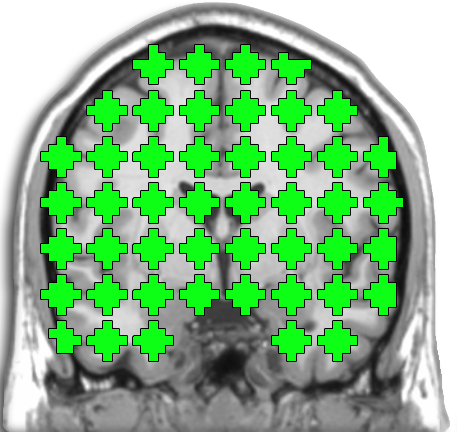
\includegraphics[height=\imheight]{roi_slice_cor.png}&
		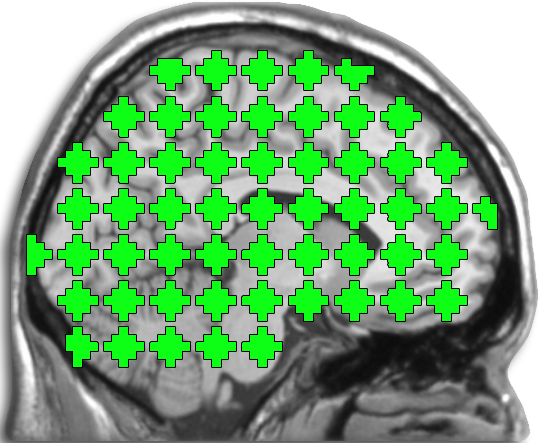
\includegraphics[height=\imheight]{roi_slice_sag.png}&
		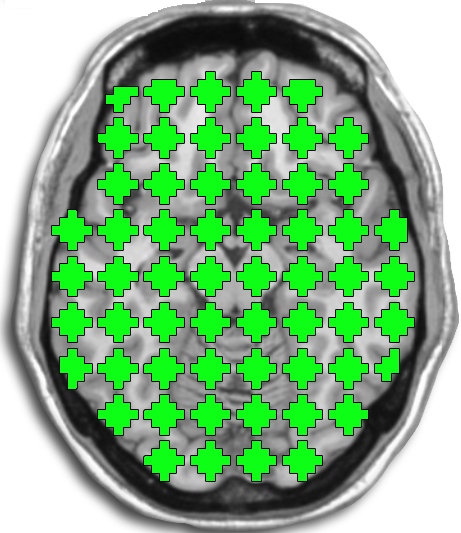
\includegraphics[height=\imheight]{roi_slice_axi.png}	\vspace{-8pt}\\
	\end{tabular}
	\caption{
	The brain parcellation scheme adopted in this work.
	The green regions represent (pseudo)-spherical nodes each encompassing $33$ voxels.
	}
	\vspace{-5pt}
	\label{fig:roi,grid,slice}
\end{figure}

%%%%%%%%%%%%%%%%%%%%%%%%%%%%%%%%%%%%%%%%%%%%%%%%%%%%%%%%%%%%%%%%%%%%%%%%%%%
% Explain L1/L2 MTL penalty
%%%%%%%%%%%%%%%%%%%%%%%%%%%%%%%%%%%%%%%%%%%%%%%%%%%%%%%%%%%%%%%%%%%%%%%%%%%
\vspace{-4pt}\subsection{Structured Sparsity with Group Variable Selection}\vspace{-2pt}
\renewcommand{\HSPACE}{\hspace{-3pt}}
\newcommand{\xx}{\xmath{\grave{x}}}
\newcommand{\yy}{\xmath{\grave{y}}}
\newcommand{\zz}{\xmath{\grave{z}}}

We propose to integrate the \emph{structured sparsity} framework introduced in~\cite{Watanabe:2014} with the popular multitask \mbox{\MTL-penalty} \cite{Obozinski:2010,Chen:2012b}.
Specifically, for the inter-task penalty \RegB, we use $\RegB(\wall){=}\sum_{j=1}^p \norm{\w_j}_2$, which is the so-called \MTL-penalty.
Here $\w_j\,{\in}\,\reals^K$ is a vector formed by stacking the \mbox{$j$-th} weight vector coefficients across the $K$  tasks.
This penalty has the appealing \emph{group variable selection} property~\cite{Obozinski:2010,Chen:2012b}, which promotes learning features that are relevant across all sites, thereby simplifying interpretation of the selected features. At the same time, the actual weights associated with a given correlation can vary across site, in contrast to training a single classifier over a pooled dataset.

%%%%%%%%%%%%%%%%%%%%%%%%%%%%%%%%%%%%%%%%%%%%%%%%%%%%%%%%%%%%%%%%%%%%%%%%%%%
% Optimization
%%%%%%%%%%%%%%%%%%%%%%%%%%%%%%%%%%%%%%%%%%%%%%%%%%%%%%%%%%%%%%%%%%%%%%%%%%%
%=========================================================================%
% admm algorithm
%=========================================================================%
\afterpage{\begin{figure}
{\begin{minipage}{0.999\textwidth}\vspace{-25pt}
\algrenewcommand\algorithmicindent{14pt} % <- (03/16/2014) change indentation http://tex.stackexchange.com/questions/47695/change-indentation-size-in-algorithmicx-package
%\setlength{\textfloatsep}{15pt}% <- to suppress annoying white-space after alg
\renewcommand{\HSPACE}{\hspace{3pt}}
\begin{algorithm}[H] % <- (06/04/2014)for somereason, adding [H] option allows "algorithm" env to be inside figure env
\floatname{algorithm}{Alg.} % <- allows me to change the caption header
\caption{ADMM for Multitask Structured Sparse SVM}
\label{alg:admm}
\renewcommand{\FSIZE}[1]{\tfontsize{9pt}{#1}}
\begin{algorithmic}[1]
\begin{spacing}{1.09}
\tfontsize{9.45pt}{\vspace{0pt}
	\State Initialize variables, assign hyperparameters $\lambda,\gamma\geq 0$\vspace{0pt}
	\Repeat\vspace{2pt}
		%%%%%%%%%%%%%%%%%      FOR LOOP     %%%%%%%%%%%%%%%%%%%%%%%%%%%%%%%%%%%%%%%%
		\For{$k=1,\dots,K$}
			%==================================================%
			% w update
			%==================================================%
			\State\HSPACE$\wk\leftarrow$
				$((\Xk)^T\Xk{+}2\I_p)\inv\big\{(\Yk\Xk)^T\left(\vak{-}\uak\right)\left(\vbk{-}\ubk\right){+}\A^T\left(\vdk{-}\udk\right)\big\}$
				\vspace{-8pt}\Statex\Comment{\FSIZE{solve using matrix inversion Lemma}}\vspace{2pt}
			
			%==================================================%
			% v3 update
			%==================================================%
			\State\HSPACE $\vck \leftarrow$
				$\begin{cases}
					\text{apply Equation \eqref{eqn:prox}} 
						& \text{if } q\,{=}\,1 \text{ (FL)}\\
					\rho(\gamma\B+\rho\I)\inv\Ctil(\vdk-\uck) 
						& \text{if } q\,{=}\,2 \text{ (GN)}\\
				\end{cases}$

			%==================================================%
			% v1 update
			%==================================================%
			\State\HSPACE $\vak {\leftarrow} \prox_{\loss/(\rho{}n_k)}\hspace{-2pt}\left(\Yk\Xk\wk{+}\uak\right)$%
%-------------------------------------------------------------------------%
\Comment{\FSIZE{%
					$\prox_{\tau\loss}(t)\,{:=}\,
						\begin{cases}
							t 		& \text{if } t > 1	\\[-3pt]
							1 		& \text{if } 1-\tau {\leq} t \,{\leq}\, 1  \\[-3pt]
							t{+}\tau\!\!\!	& \text{if } t < 1-\tau
						\end{cases}
						\nonumber
					$}}
%-------------------------------------------------------------------------%
			\vspace{-1pt}
			%==================================================%
			% v4 update
			%==================================================%
			\State\HSPACE $\vdk \leftarrow 
				\big(\Ctil'\Ctil{+}\I_\ptil\big)\inv
				\big(\Ctil'[\vck+\uck]{+}\A\wk{+}\udk\big)$ 
				\Comment{\FSIZE{solve using FFT}}\vspace{5.0pt}
		\EndFor
		%%%%%%%%%%%%%%%%%%%%%%%%%%%%%%%%%%%%%%%%%%%%%%%%%%%%%%%%%%%%%%%%%%%%%%%%%%%

		\vspace{4pt}
		%=================================================================%
		% v2 update
		%=================================================================%
		\For{$j=1,\dots,p$}
		\State\HSPACE $\vbj \leftarrow 
			\vsoft_{\lambda/\rho}\left(\wj+\ubj\right)$%
			%-------------------------------------------------------------------------%
\Comment{\FSIZE{$\text{vsoft}_{\tau}(\bmath{t}){:=}\text{max}(1-\frac{\tau}{\norm{\bmath{t}}_2},0) \,\bmath{t},\;\;\bmath{t}\,{\in}\,\reals^K$}}
			%-------------------------------------------------------------------------%
		\EndFor

		\vspace{4pt}
		%=================================================================%
		% dual update
		%=================================================================%
		\For{$k=1,\dots,K$}\Comment{dual variable update}\vspace{1.75pt}
			\State\HSPACE $\uak \leftarrow \uak + \Yk\Xk\wk-\vak$\vspace{1.75pt}
			\State\HSPACE $\ubk \leftarrow \ubk + \wk - \vbk$\vspace{1.75pt}
			\State\HSPACE $\uck \leftarrow \uck + \vck - \Ctil\vdk$\vspace{1.75pt}
			\State\HSPACE $\udk \leftarrow \udk + \A\wk - \vdk$\vspace{1.75pt}
		\EndFor\vspace{0pt}
	\Until{stopping criterion is met}
}
\vspace{-0.045\linewidth}\end{spacing}
\end{algorithmic}
\end{algorithm}
%%%%%%%%%%%%%%%%%%%%%%%%%%%%%%%%%%%%%%%%%%%%%%%%%%%%%%%%%%%%%%%%%%%%%%%%%%%
%%%%%%%%%%%%%%%%%%%%%%%%%%%%%%%%%%%%%%%%%%%%%%%%%%%%%%%%%%%%%%%%%%%%%%%%%%%
%%%%%%%%%%%%%%%%%%%%%%%%%%%%%%%%%%%%%%%%%%%%%%%%%%%%%%%%%%%%%%%%%%%%%%%%%%%
\end{minipage}}
\vspace{-22pt}
\end{figure}
}

\vspace{-4pt}\subsection{Optimization Algorithm}\vspace{-2pt}
To solve the proposed large scale optimization problem, we apply the \emph{alternating direction method of multipliers} (ADMM) algorithm \cite{Boyd:2011} introduced in \cite{Watanabe:2014}, but with a minor modification.
The complete algorithm is outlined in Alg.~1.
We note that this section focuses on GN and FL, but the ADMM algorithm for TV differs only in line~5 of Alg.~1, but the details are omitted for lack of space.

To apply Alg.~1, we employ the \emph{data augmentation}${+}$\emph{masking} strategy that was proposed in \cite{Watanabe:2014}.
In brief, the idea behind this method is that as it stands, the ADMM algorithm for solving the objective function~\eqref{eqn:erm2} with the GN, FL, or TV penalty will require the inversion of the Laplacian matrix $\C^T\C$, which~is prohibitively large.
Thus we rewrite the GN/FL penalty as $\RegA(\wk){=}\|\B\Ctil\A\wk\|^q_q\,$, where \A is an \emph{augmentation \mbox{matrix}}, \Ctil is the finite differencing matrix for the augmented \wk, 
and \B is a diagonal masking matrix that ensures the penalty remains unaffected, \ie, $\|\B\Ctil\A\wk\|^q_q\;{=}\,\|\C\wk\|^q_q$.
This results in a new Laplacian matrix $\Ctil^T\Ctil$, which possesses a special structure known as \emph{block-circulant with circulant-blocks}, whose matrix inverse can be evaluated efficiently via the fast Fourier Transform (FFT) (line 7, Alg.~1; see~\cite{Watanabe:2014} for more details). 

\hspace{-1pt}Using this augmentation$+$masking strategy, we can rewrite the objective as:
\begin{equation}
		\min_{\wall} 
			\sum_{k=1}^K\hspace{-0pt}\frac{1}{n_k}\Loss(\Yk\Xk\wk){+}
			\frac{\gamma}{q}\hspace{-0pt}\sum_{k=1}^K\hspace{-1pt}
			\big\|\B\Ctil\A\wk\big\|_q^q\hspace{-0pt}{+}
			\lambda\hspace{-0pt}\sum_{j=1}^p\norm{\w_j}_2 \;,  
	\nonumber
\end{equation}
which can be converted into the following canonical ADMM form \hspace{-1.5pt}\cite{Boyd:2011}:\hspace{-1.5pt}
\begin{equation}
		\displaystyle\min_{\{\wk, \vak, \vbk, \vck, \vdk\}} 
			\sum_{k=1}^K\frac{1}{n_k}\Loss(\vak) + 
			\frac{\gamma}{q}\sum_{k=1}^K\norm{\B\vck}_q^q + 
				\lambda\sum_{j=1}^p\norm{\bmath{v_{2,j}}}_2
 \; 
	\nonumber
\vspace{-3pt}\end{equation}
\begin{equation}\vspace{-5pt}
		\text{ s.t. }  \Yk\Xk\wk{=}\vak,\wk{=}\vbk,  \Ctil\vdk{=}\vck,  \A\wk{=}\vdk \quad \forall k\,{=}\,1,\dots,K.
	\label{eqn:admm,splitting2}
\end{equation}
It is straightforward to show that the above two problems are equivalent, and Alg.~1 follows from applying the standard ADMM iteration on \eqref{eqn:admm,splitting2}.
We emphasize that all the updates in Alg.~1 can be carried out efficiently in analytical form.
\newcommand{\IDX}{s}
For example, line~5 in Alg.~1 is a simple diagonal matrix inversion in the case of GN, and for the FL case we have the following closed form update:
\vspace{-1pt}\begin{equation}\vspace{-1pt}
	\left[\vck\right]_\IDX \;\leftarrow
	\begin{cases}
		\soft_{\gamma/\rho}\Big(\big[\Ctil(\vdk-\uck)\big]_\IDX\Big) 
			& \text{if } \B_{\IDX,\IDX}=1 \\
		\big[\Ctil(\vdk-\uck)\big]_\IDX & \text{if } \B_{\IDX,\IDX}=0,
	\end{cases}
\label{eqn:prox}
\end{equation}
where  
$\text{soft}_{\tau}(t){:=}\text{max}(1\,{-}\,\frac{\tau}{\abs{t}},0)\,{\cdot}\,t$
denotes the \emph{soft-threshold operator} and $\left[\cdot\right]_\IDX$ indexes the $\IDX$-th element of a vector.
Finally, we note $\text{Prox}_{\tau\loss}(t)$ in line~6 is an elementwise update corresponding to the proximal operator of the hinge-loss.
